\chapter{Flow of Associations and Causal Graphs}

In un grafo diretto indichiamo con $pa(X)$ i \textbf{genitori} del nodo $X$ e $ch(Y)$ i \textbf{figli} del nodo $Y$.

\begin{center}
  \begin{minipage}[c]{0.5\linewidth}
    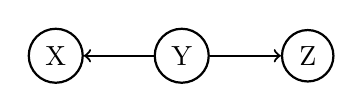
\begin{tikzpicture}[node distance={16mm}, thick, main/.style = {draw, circle}]
      \node[main] (1) {X};
      \node[main] (2) [right of=1] {Y};
      \node[main] (3) [right of=2] {Z};
      \draw[<-] (1) -- (2);
      \draw[->] (2) -- (3);
    \end{tikzpicture}
  \end{minipage}
  %
  \begin{minipage}[c]{0.4\linewidth}
    \setlength{\abovedisplayskip}{0pt}
    \begin{flalign*}
      &pa(Y) = \emptyset&  ch(Y) &= \{X,Z\}&\\
      &pa(X) = Y& ch(X) &= \emptyset&
    \end{flalign*}
  \end{minipage}
\end{center}

Un \textbf{cammino} è una qualsiasi sequenza di nodi adiacenti, indipendentemente dalla direzione degli archi che li collega.

Un \textbf{cammino diretto} è un qualsiasi \textbf{cammino} tra due nodi in cui tutti gli archi che li collega hanno la stessa direzione.

$de(Y)$ è l'insieme dei nodi \textbf{discendenti} del nodo $Y$, ovvero tutti i nodi che possono essere raggiunti da $Y$.

$an(Z)$ è l'insieme dei nodi \textbf{antenati} del nodo $Z$, ovvero tutti i nodi che da $Z$ possono essere raggiunti.

\begin{center}
  \begin{minipage}[c]{0.4\linewidth}
    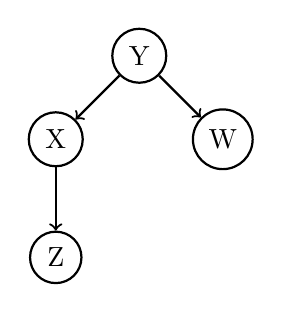
\begin{tikzpicture}[node distance={15mm}, thick, main/.style = {draw, circle}]
      \node[main] (1) {Y};
      \node[main] (2) [below left of=1] {X};
      \node[main] (3) [below right of=1] {W};
      \node[main] (4) [below of=2] {Z};
      \draw[->] (1) -- (2);
      \draw[->] (1) -- (3);
      \draw[->] (2) -- (4);
    \end{tikzpicture}
  \end{minipage}
  \begin{minipage}[c]{0.3\linewidth}
    $an(Z) = \{X, Y\}$\\
    $an(Y) = \emptyset$

    \bigskip
    $de(Y) = \{X, Z, W\}$\\
    $de(W) = \emptyset$
  \end{minipage}
\end{center}

\section{Bayesian Networks}
In una rete bayesiana vogliamo modellare la distribuzione di probabilità $P(X_1, \dots, X_n)$.
Tramite la \textbf{Chain Rule} possiamo riscriverla nel seguente modo:
\begin{flalign*}
  P(X_1, \dots, X_n) &= P(X_1)P(X_2|X_1)P(X_3|X_1,X_2) \cdot\cdot\cdot P(X_n|X_1, \dots, X_{n-1}) & \\
  &= P(X_1)\prod_{i=2}^n{P(X_i|X_1, \dots, X_{i-1})} &
\end{flalign*}
%
\textbf{Local Markov Assumption}:
Un nodo $X$ è indipendente da tutti i suoi non-discendenti date l'evidenze di tutti i nodi genitori $pa(X)$.

Data questa assunzione possiamo applicare la fattorizzazione della probabilità $P$.
\begin{flalign*}
  &P(X_1, \dots, X_n) = \prod_{i=1}^n{P(X_i|pa(X_i)})&
\end{flalign*}
%
In questo modo possiamo ridurre il numero di parametri della rete.

Una distribuzione di probabilità $P$ si dice che sia Markov se ogni nodo $X$ rispetta la Local Markov Assumption.

L'assunzione di Markov non ci da informazioni riguardo relazioni di dipendenza tra i nodi.
Quindi estendiamo quest'assunzione.

\textbf{Minimality Assumption}
\begin{itemize}
  \item Dato $pa(X)$, un nodo $X$ è indipendente da tutti i suoi non-discendenti.
  \item I nodi adiacenti sono dipendenti.
\end{itemize}

Dato un DAG $G$, se $P$ è Markov allora sappiamo:
\begin{itemize}
  \item $P$ soddisfa un insieme di indipendenze specificate dalla struttura di $G$.
  \item se $P$ soddisfa pure la Minimality Assumption, allora l'insieme di indipendenze è minimale,
        ovvero $P$ non soddisfa altre indipendenze in $G$.
        Questo equivale a dire che tutti i nodi adiacenti sono dipendenti.
\end{itemize}

\section{Causal Networks}

Una variabile $X$ si dice \textbf{causa} di una variabile $Y$ se $Y$ può
cambiare in risposta a un cambiamento di $X$.

\textbf{Causal Edge Assumption}:
Ogni variabile associata a un nodo è causata dalle variabili dei nodi genitori.

Un \textbf{Grafo Causale} è un DAG in cui è soddisfatta la proprietà \textbf{Causal Edge Assumption}.

\begin{center}
  \begin{minipage}[c]{0.3\linewidth}
    \vspace{0pt}\
    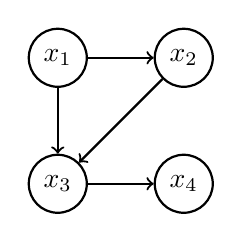
\begin{tikzpicture}[node distance={16mm}, thick, main/.style = {draw, circle}]
      \node[main] (1) {$x_1$};
      \node[main] (2) [right of=1] {$x_2$};
      \node[main] (3) [below of=1] {$x_3$};
      \node[main] (4) [right of=3] {$x_4$};
      \draw[->] (1) -- (2);
      \draw[->] (1) -- (3);
      \draw[->] (2) -- (3);
      \draw[->] (3) -- (4);
    \end{tikzpicture}
  \end{minipage}
  %
  \begin{minipage}[c]{0.4\linewidth}
    $X_1$ causa direttamente $X_2$ e $X_3$\\
    $X_2$ causa direttamente $X_3$\\
    $X_3$ causa direttamente $X_4$

    \bigskip
    $X_1$ causa indirettamente $X_4$
  \end{minipage}
\end{center}
\bigskip

Per capire la differenza tra association flow e causation flow utilizziamo dei grafi elementari.

\begin{figure}[h]
  \centering

  \begin{subfigure}[c]{0.34\linewidth}
    \centering
    \bigskip
    \bigskip
    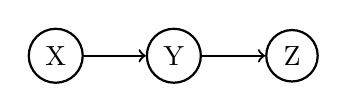
\begin{tikzpicture}[node distance={15mm}, thick, main/.style = {draw, circle}]
      \node[main] (1) {X};
      \node[main] (2) [right of=1] {Y};
      \node[main] (3) [right of=2] {Z};
      \draw[->] (1) -- (2);
      \draw[->] (2) -- (3);
    \end{tikzpicture}
    \bigskip
    \caption{Chain}
  \end{subfigure}
  %
  \begin{subfigure}[c]{0.32\linewidth}
    \centering
    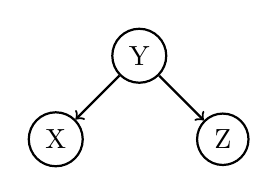
\begin{tikzpicture}[node distance={15mm}, thick, main/.style = {draw, circle}]
      \node[main] (2) {Y};
      \node[main] (1) [below left of=2] {X};
      \node[main] (3) [below right of=2] {Z};
      \draw[->] (2) -- (1);
      \draw[->] (2) -- (3);
    \end{tikzpicture}
    \caption{Fork}
  \end{subfigure}
  %  
  \begin{subfigure}[c]{0.32\linewidth}
    \centering
    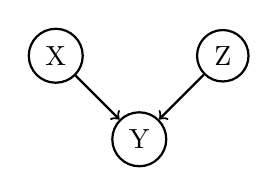
\begin{tikzpicture}[node distance={15mm}, thick, main/.style = {draw, circle}]
      \node[main] (2) {Y};
      \node[main] (1) [above left of=2] {X};
      \node[main] (3) [above right of=2] {Z};
      \draw[->] (1) -- (2);
      \draw[->] (3) -- (2);
    \end{tikzpicture}
    \caption{Collider}
  \end{subfigure}
\end{figure}

Il flusso di associazione esprime che due nodi del grafo sono associati o meno.

Vogliamo sapere se due nodi sono (statisticamente) dipendenti o indipendenti.

\subsubsection*{Un-connected Nodes}
Due nodi sconnessi non sono associati. Questo può essere dimostrato applicando la fattorizzazione.
%
\begin{align*}
  P(X, Y) & = P(X | Y) P(Y)             \qquad & \text{(probabilità composta)} \\
          & = P(X | pa(X)) P(Y | pa(Y)) \qquad & \text{(fattorizzazione)}      \\
          & = P(X) P(Y)                 \qquad & \text{indipendenza}
\end{align*}

Due nodi connessi adiacenti sono dipendenti per la \textbf{local edge assumption}.

\subsubsection*{Chain e Fork}


\subsubsection*{Collider}


\section{D-Separation}
Un percorso $p$ si dice bloccato da un insieme di nodi $S$ sse
\begin{itemize}
  \item $p$ contiene una chain $A \rightarrow B \rightarrow C$ o una fork $A \leftarrow B \rightarrow C$ e $B \in S$
  \item $p$ contiene un collider $A \rightarrow B \leftarrow C$ e $B \notin S, de(B) \nsubseteq S$
\end{itemize}
Se l'insieme $S$ blocca ogni percorso tra due nodi $X$ e $Y$, allora $X$ e $Y$ si dicono \textbf{d-separati} da $S$,
e quindi indipendenti dato $S$.

ESEMPI...

La d-separazione implica l'indipendenza condizionale.

\begin{itemize}
  \item Due variabili $X$ e $Y$ sono d-separate nel grafo $G$ \\quando condizionate dall'insieme $S$ ($X \ind_G Y | S$).
  \item Due variabili $X$ e $Y$ sono indipendenti nella distribuzione $p$ \\quando condizionate dall'insieme $S$ ($X \ind_p Y | S$).
\end{itemize}

$X \ind_G Y | S \Rightarrow X \ind_p Y | S$
